\graphicspath{{./figures}}

\section{PocketQube}

The PocketQube standard is a fairly new set of protocols and specifications defining a modularized nano-satellite system. The term \textit{modularized} in this context refers to the ability for different "modules" or PocketQube units, each with their own set functionality, to be connected to a common \textit{backplane} and integrated seamlessly. \textit{Integration} here refers to both the mechanical spacing of each module, as well as the electronic communication between the modules.

\begin{figure}[!htb]
    \centering
    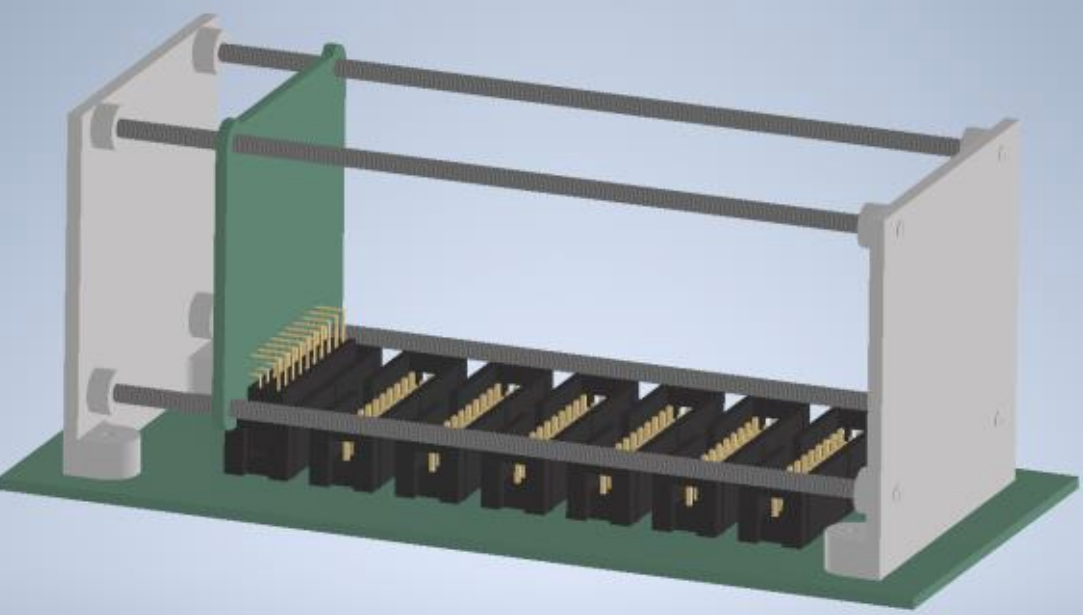
\includegraphics[width=0.6\textwidth]{pq_enclosure}
    \caption{A PQSU Enclosure \cite{standard-pqsu}}
    \label{fig:pq_enclosure}
\end{figure}

As an example, a PocketQube enclosure could contain three units: a communication module, a sensor pack, and a battery system. These modules can then be connected onto the backplane via headers, and placed inside a single enclosure, such as that in Figure \ref{fig:pq_enclosure}. This "nano-satellite" can then be "launched" through any means.